\chapter{The Good Citizen}

These notes follow Michael Sandel's tenth lecture in the Justice course, curated here by LazyingArt LLC. We begin where the lecture begins: with a deliberate turn away from Kant and Rawls and toward Aristotle. From there Sandel does not remain at the level of abstraction. He moves from the compact case of flutes to the larger case of politics, then to the Casey Martin golf-cart controversy, and only after those examples are in place does he raise the deepest objection, namely whether a teleological account of justice leaves room for freedom. The order is essential. Each step prepares the next.

\section{From Rawls and Kant to Aristotle}

Sandel opens by recalling what modern theories of justice often try to do: detach justice and rights from questions of virtue and moral desert. Aristotle refuses that separation. On his view, justice concerns what people deserve, and so the argument over justice cannot be settled until we know what sort of thing is being distributed and what it is for.

\begin{equation}
\text{justice}=\text{giving people what they deserve}
\end{equation}

That is Sandel's first Aristotelian formula. But he does not let it sit as a slogan. The lecture immediately presses on the hidden difficulty inside it. To say that justice gives people what they deserve is not yet to say what counts as desert. We still need the relevant respect in which one person rather than another deserves the good.

\begin{definition}
A teleological account of justice asks what a practice, institution, or good is for before deciding how it should be distributed. The telos of the thing fixes the relevant criterion of merit.
\end{definition}

This point is more exact than it first appears. Aristotle is not saying that every practice has the same end, or that one moral vocabulary can be imposed indiscriminately everywhere. He is saying that the distribution of any good already presupposes an answer, whether acknowledged or not, to the question what that good is for.

\subsection{Question \& Answer}

Why is bare equality not enough?

Because the formula of equality is incomplete until we specify the relevant dimension of comparison. Equal things should go to equal persons, yes. But equal with respect to what? Aristotle's answer, as Sandel presents it, is that we discover the relevant respect by looking to the characteristic end or purpose of the thing distributed.

\begin{align}
\text{equal things} &\Longrightarrow \text{equal persons},\\
\text{equal in what respect?} &\Longrightarrow \text{look to the telos of the thing distributed}.
\end{align}

Once we see this, the lecture acquires its shape. Equality is not discarded; it is interpreted. The missing middle term is telos.

\section{Flutes, Telos, and the Honorific Turn}

Sandel next turns to Aristotle's example of flutes. The move is methodical. Before we approach politics, rights, and law, we are given a small, almost schematic case where the logic can be seen clearly. Who should get the best flutes? Aristotle's answer: the best flute players.

\begin{equation}
\text{best flutes} \Longrightarrow \text{best flute players}
\end{equation}

\paragraph{A worked Aristotelian example.}

The point becomes clearer if we write the example in stages:

\begin{align}
\text{thing distributed} &= \text{flutes},\\
\text{telos} &= \text{good flute playing},\\
\text{relevant excellence} &= \text{excellence in flute playing},\\
\text{just recipient} &= \text{best flute players}.
\end{align}

This is the lecture's first explicit worked structure. We do not begin from private preference, or even from a thin rule of equal access. We begin from the nature of the good itself, and only then ask what excellence is relevant to its proper use.

\subsection{Question \& Answer}

Why should the best flutes go to the best flute players?

Sandel's answer is stronger than the merely instrumental claim that this will produce better music. To distribute the best flutes to the best players is also to honor the excellence internal to the practice.

\begin{equation}
\text{rewarding the great flute player}
\Longleftrightarrow
\text{honoring the excellence of flute playing}
\end{equation}

Here the lecture makes its first major expansion. Questions of distribution are also questions of recognition. The dispute is never only about who gets the object. It is also about what human quality is being singled out for esteem.

\begin{equation}
\text{debates about telos}
\Longrightarrow
\text{debates about honor}
\end{equation}

That is why the flute example matters so much. It is not a decorative illustration. It installs the method that will govern the rest of the lecture and introduces the honorific dimension that will return in politics and again in sport.

We can compress the structure Sandel has now built in the following schematic:

\begin{figure}
\centering
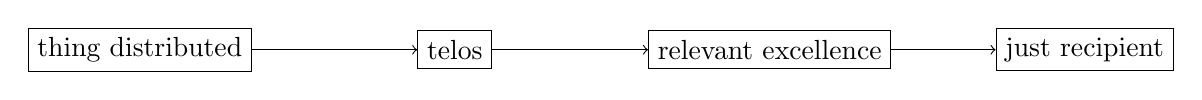
\begin{tikzpicture}
\node (a) [draw, rectangle] at (0,0) {thing distributed};
\node (b) [draw, rectangle] at (4,0) {telos};
\node (c) [draw, rectangle] at (8,0) {relevant excellence};
\node (d) [draw, rectangle] at (12,0) {just recipient};
\draw[->] (a) -- (b);
\draw[->] (b) -- (c);
\draw[->] (c) -- (d);
\end{tikzpicture}
\end{figure}

Only after this compact model is in place does Sandel widen the frame. It is not easy, he says, to dispense with teleological reasoning in ethics, justice, and moral argument. To bring out the force of Aristotle's claim, he will consider two larger examples: politics and golf.

\section{Politics as the Distribution of Offices and Honors}

The first large example is politics. Sandel marks an important contrast here. When we speak of distributive justice now, we usually have in mind the distribution of income, wealth, and opportunity. Aristotle's focus is different. He is mainly concerned with offices, citizenship, honors, and political rule.

\begin{align}
\text{modern distributive justice}
&\approx
\text{income}+\text{wealth}+\text{opportunity},\\
\text{Aristotelian distributive justice}
&\approx
\text{offices}+\text{honors}+\text{political rule}.
\end{align}

That shift in subject matter changes everything. If politics is about rule, then before we decide who should rule we must first ask what politics is for. Sandel keeps the order exact: telos first, distribution second.

Aristotle's answer is that politics is about forming character, cultivating the virtue of citizens, and realizing the good life. The political community is not merely an arrangement for coexistence. It is an association ordered to a certain human good.

\begin{align}
\text{telos of politics}
&=
\text{forming character}
+\text{cultivating virtue}
+\text{good life},\\
\text{mere life},\ \text{economic exchange},\ \text{security}
&\neq
\text{end of the polis},\\
\text{end of the polis}
&=
\text{good life}.
\end{align}

Sandel immediately lets the modern worry surface. Perhaps, one might say, this is precisely why Kant and Rawls are right. Politics should not make us good. It should secure the freedom of persons to choose their own ends, consistent with a similar liberty for others. Aristotle disagrees. A polis that does not aim at goodness is, in his view, only a nominal polis. It sinks into a mere alliance, and law becomes a covenant protecting individuals from one another rather than a mode of common life that makes citizens good and just.

\subsection{Question \& Answer}

If politics is for the good life, who should rule?

Aristotle's answer follows the same teleological structure we saw with flutes. If the political community exists for the good life, then the criterion of political distribution must be contribution to that end.

\begin{align}
\text{telos of politics}
&\Longrightarrow
\text{criterion for distributing political authority},\\
\text{criterion for distributing political authority}
&=
\text{contribution to the good life of the polis},\\
\text{those who contribute most to the good life of the polis}
&\Longrightarrow
\text{greater share in rule and honor}.
\end{align}

Sandel is careful at this point not to let the argument collapse into a simple claim about outcomes. It is true that those with the best judgment may govern best. But there is a further reason, and it is distinctively Aristotelian: politics is itself an arena in which civic excellence is honored. Rule is not only a tool for producing consequences; it is also a public recognition of virtue.

\section{Why Political Life Matters to Human Flourishing}

At this stage Sandel raises the natural question. Why should political participation be essential to living well? Why can a person not live a morally decent, even admirable, life outside politics?

He says Aristotle gives two answers, and the lecture preserves the difference between them. The first answer is preliminary and comes from the Politics. Human beings are by nature political. We fully realize our nature only in a polis, because only there do we fully exercise the specifically human capacity for language understood as deliberation about right and wrong, justice and injustice.

\begin{align}
\text{human beings by nature}
&\Longrightarrow
\text{polis},\\
\text{isolated human being}
&\Longrightarrow
\text{beast or god}.
\end{align}

Sandel is precise here. The polis is prior to the individual not in time but in purpose. A solitary human being may survive, but cannot fully unfold the capacities that are constitutive of human life as such.

Then comes the fuller answer, drawn from the Nicomachean Ethics. Happiness is not simply the favorable balance of pleasure over pain. It is an activity of the soul in accordance with virtue.

\begin{equation}
\text{happiness}
=
\text{activity of the soul in accordance with virtue}
\end{equation}

Once this is said, the connection between ethics and politics becomes tighter. If happiness is an activity of virtue, then the shaping of character cannot be politically irrelevant. Sandel emphasizes that every serious student of politics must therefore study the soul, because legislation in a good city aims, at least in part, at moral formation.

But now another question arises. Why can virtue not be learned from rules alone? Why can we not simply learn sound principles, whether at home, in a classroom, or from a book, and then apply them?

\begin{align}
\text{virtue} &\neq \text{book learning only},\\
\text{virtue} &\sim \text{practice},\\
\text{practice} &\Longrightarrow \text{discerning particulars}.
\end{align}

This is where Sandel lingers over examples that are easy to understate: flute playing, cooking, joke telling. No one becomes an accomplished musician, chef, or comedian by memorizing precepts alone. These are activities of judgment. We learn them by doing, by getting the hang of them, and above all by learning to discern the particulars of situations. Aristotle, as Sandel presents him, thinks virtue is learned in just this way.

\subsection{Question \& Answer}

Why can we not live a fully good life outside politics?

Because the virtues are not merely inward states. They are formed in practice, and one of the practices necessary to the human good is deliberation with fellow citizens about justice and the good. Sandel's two-step answer may be written compactly as follows:

\begin{enumerate}
\item Human beings realize their nature through language and deliberation.
\item Deliberation about just and unjust belongs to political life.
\item Happiness is activity in accordance with virtue.
\item Virtue is acquired by practice and habituation.
\item Therefore participation in a political community is part of the way human excellence is formed.
\end{enumerate}

The lecture then returns from ethics to institutions. If civic virtue is the excellence politics most centrally calls forth, then those who possess civic virtue most fully deserve the greatest share of political office and honor. Sandel's emblematic figure here is Pericles.

\begin{equation}
\text{civic virtue}
\approx
\text{deliberating among equals}
\end{equation}

\begin{equation}
\text{Pericles / greatest civic virtue}
\Longrightarrow
\text{greatest measure of offices and honors}
\end{equation}

Again, the argument is not exhausted by consequences. Pericles should not merely have influence because he may produce better results. Politics also honors the citizen who best embodies civic excellence and practical wisdom. That is the honorific dimension of Aristotle's politics.

\section{Casey Martin, Golf, and the Telos of a Game}

Only after the politics example is complete does Sandel turn to the second case, the controversy over Casey Martin and the golf cart. The transition is exact. He introduces the case as another way to bring out the force of Aristotle's claim. Rights arguments, he says, may depend on prior arguments about telos; and disputes over telos often turn out also to be disputes over honor.

Casey Martin is a gifted golfer who can compete at the highest level except for one obstacle: he suffers from a rare circulatory condition that makes walking difficult and dangerous. He asks the PGA to let him use a cart during professional tournaments. The PGA refuses. He sues, and the case reaches the Supreme Court. Sandel then does something important pedagogically: he polls the room. From a moral point of view, should Martin have a right to a cart?

The classroom responses are divided. One line of argument says that walking the course has been intrinsic to golf since the inception of the sport, especially at the professional level. Another line says that even with a cart Martin continues to walk a significant amount and continues to suffer more pain and fatigue than a healthy player. The accommodation does not remove disadvantage so much as reduce it.

\subsection{Question \& Answer}

Does Casey Martin have a right to use a golf cart, or does that depend on the purpose of golf?

Sandel's Aristotelian answer is that the right depends on the purpose. That is precisely the point of choosing this example.

\begin{align}
\text{rights claim in golf}
&\Longrightarrow
\text{depends on the telos of golf},\\
\text{walking essential to golf?}
&\Longrightarrow
\text{Casey Martin right to cart?}
\end{align}

This is one of the lecture's most important practical tests. If walking is essential to the game, then Martin's claim weakens. If walking is not essential, then the case for accommodation strengthens. Either way, the argument about rights cannot be decided without an argument about what golf is.

Sandel then brings in the judicial contrast. The Court's majority, as he reports it, held that walking is not an essential part of golf. The physical burden, they suggest, is limited enough that the central point of the game lies elsewhere. Justice Scalia dissents, and his dissent matters because it is not merely a different answer within Aristotle's framework. It is a rejection of the framework itself.

\begin{equation}
\text{game}=\text{mere amusement}
\end{equation}

This is Scalia's anti-Aristotelian position as Sandel presents it. A game has no objective purpose to be discovered. It exists for amusement, and different groups may organize different versions of it as they please. The market, not a court and not some philosophical inquiry into essence, will determine which versions people care about.

Sandel is not persuaded. The very fact that the case becomes a debate over whether walking is essential already shows that teleological questions reappear even when we try to avoid them. And beneath the explicit dispute, he says, something else is rumbling: whether walking partly determines whether golf counts as a genuine athletic competition rather than only a game of skill.

\section{The Recap Seam: Fairness and the Honor of Sport}

When the lecture returns to the golf case, it does so across a visible seam. Sandel says: when we ended last time, we were debating whether Casey Martin had a right to ride in a golf cart. He briefly restates the larger philosophical stakes. Aristotle's view is teleological because it ties rights to the purpose of a practice, and it is also a theory of justice as fit because it fits persons and excellences to appropriate roles.

\begin{equation}
\text{justice as fit}
=
\text{fitting persons with virtues/excellences to appropriate roles}
\end{equation}

That restatement is not redundant. It prepares the deepening of the case. We are no longer only asking whether Martin should receive an accommodation. We are asking how the case illuminates Aristotle's whole conception of justice.

The pressure point now comes from Jenny's proposal. Why not simply make carts available to everyone? If the objection is unfair advantage, let every golfer decide whether to walk or ride.

\subsection{Question \& Answer}

Would allowing everyone to use a cart solve the fairness problem, or would it change the game?

This is where the lecture becomes especially vivid. Da replies with the flippers analogy: if we allow everyone to use flippers in swimming, we may achieve one kind of symmetry while destroying the athletic point of the sport. Jenny responds that excluding a golfer who is passionate, highly skilled, and capable of competing may itself betray the spirit of the game. Michael insists that the PGA is the pinnacle and that its standards define what it takes to belong there.

The exchange allows Sandel to draw out two morals. The first is the one already visible in the first pass through the case: Martin's right depends on whether walking is essential to golf. The second is more revealing. The controversy is not only teleological. It is honorific.

\begin{equation}
\text{golf controversy}
\Longrightarrow
\text{teleological dispute}+\text{honorific dispute}
\end{equation}

Why are professional golfers so resistant not only to Martin's cart but even to Jenny's universal-cart proposal? Sandel's answer is dry and pointed: professional golfers are sensitive about whether their sport is really a sport. If everyone may ride in a cart, golf begins to look less like an athletic competition and more like a game of skill. What is at stake is not only the rulebook. It is the public honor attached to a certain kind of excellence.

\begin{equation}
\text{sport as practice}
\Longrightarrow
\text{calls forth and honors certain excellences}
\end{equation}

This is Sandel's answer to Scalia. Sports are not mere amusement. They are also objects of appreciation. They call forth excellences, prize them, and make it intelligible to argue over which features are central and which are incidental. The dispute over walking is therefore also a dispute over what golf recognizes and rewards.

The lecture has now completed the parallel Sandel announced earlier. Politics and golf are very different domains, but each shows the same structure. A question of justice leads to a question of purpose, and the question of purpose turns out to involve a question of honor.

\section{Freedom, Slavery, and the Objection to Teleology}

Only after flutes, politics, and golf are in place does Sandel turn explicitly to evaluation. He asks whether Aristotle's theory of justice is persuasive, but he does not begin from nowhere. He first anticipates the most obvious and important objection: if justice is a matter of fit between persons and roles, does that leave room for freedom?

\begin{equation}
\text{teleology}
\Longrightarrow
\text{freedom objection}
\end{equation}

The danger is plain. If a social role is said to fit my nature, where is my right to choose otherwise? If justice is tied to a substantive account of the good, what happens in a pluralist society where citizens disagree about the good?

Sandel then chooses the hardest case from Aristotle's own writings: slavery. Aristotle's defense of slavery, as reconstructed in the lecture, imposes two conditions. Slavery must be necessary for the functioning of the polis, and it must be fitting by nature for those enslaved.

\begin{align}
\text{slavery just}
&\Longrightarrow
\text{necessary} \land \text{fitting by nature},\\
\text{actual Athenian slavery}
&\not\Longrightarrow
\text{natural fit},\\
\text{coercion}
&\Longrightarrow
\text{evidence of misfit / not natural}.
\end{align}

The lecture is careful not to overstate what this shows. Sandel's point is not that Aristotle's theory contains no standards by which it may be judged. On the contrary, Aristotle's own standards condemn his own application. Many actual slaves in Athens were war captives, enslaved by luck and force rather than by any natural fitness for servitude. If coercion is needed to force a person into a role, that is strong evidence that the role is not fitting for that person. So the practice, as it existed, fails the criterion of fit.

This is why the slavery case matters. It does not merely show that Aristotle's application is morally abhorrent, though it is. It also shows that the theory can generate an internal criticism of that application. But Sandel does not let this become a vindication of Aristotle. The larger problem remains: even if some applications fail, does the teleological mode of reasoning itself threaten freedom?

\subsection{Question \& Answer}

If justice depends on telos and fit, what room is left for freedom and individual choice?

Sandel lets the student objections do much of the work here. One student caricatures the view by imagining that if a person looks and talks like a pirate, then justice must assign him to piracy rather than investment banking. Another says that even if she would be the best janitor in the world, she may want a different life. Patrick raises the broadest challenge of all: if even the contained dispute over whether walking is essential to golf yields no agreement, how can we hope to agree on the purposes of political community?

Sandel treats these objections as serious and cumulative. Much modern political theory, he says, begins exactly from this worry about disagreement over the good. Kant and Rawls conclude that rights and justice should not be grounded in any particular conception of the good life. To be free, on that view, is to stand back from our roles, traditions, and inherited purposes and to choose our ends for ourselves.

The lecture therefore closes in the right place: not with a neat decision for Aristotle or for liberal neutrality, but with the two larger questions that now frame the next step.

\begin{equation}
\text{right prior to good?}
\qquad
\text{chooser of ends vs discoverer of nature}
\end{equation}

That is not a conclusion in the ordinary sense. It is the lecture's final opening. We have now seen both the force of Aristotle's teleology and the weight of the freedom-based objection to it.

\section{Summary}

Sandel begins by turning from Kant and Rawls to Aristotle and by giving us a compact formula: justice gives people what they deserve. He then refuses to leave the formula abstract. The flute example shows that the relevant standard of desert is fixed by the telos of the thing distributed. Politics enlarges that schema into a theory of offices, honors, civic virtue, and the good life, while also bringing the modern liberal objection into view. The discussion of human flourishing deepens the point by showing why virtue, for Aristotle, must be practiced rather than merely known. The Casey Martin case then brings the same structure into a contemporary dispute about rights, fairness, and the purpose of a sport, and the resumed discussion around Jenny's proposal reveals why teleological disputes are also honorific disputes. Finally, the lecture turns to freedom and slavery, not to settle the matter, but to sharpen the confrontation between two traditions: one that ties justice to the good, and one that insists that the right must stand prior to it.